\documentclass[10pt]{article}
\newcommand{\HRule}{\rule{\linewidth}{0.5mm}}
\parindent 0pt
\parskip 10pt
\usepackage{anysize}
\usepackage{graphicx}
\usepackage{epsfig}
\usepackage{float}
%\usepackage{cite}
\usepackage{natbib}
\usepackage{setspace}
\marginsize{3.5cm}{3.5cm}{1cm}{1cm}
\onehalfspacing
\usepackage{caption}
\usepackage{subcaption}
\usepackage{amsmath,hyperref}

\usepackage{xcolor}
\hypersetup{
    colorlinks,
    linkcolor={red!50!black},
    citecolor={blue!50!black},
    urlcolor={blue!80!black}
}

%\textwidth 15cm
%\textheight 24cm
%\onehalfspacing
\begin{document}

\title{Corners Challenge}

\author{David Starkey}

\maketitle





\section{Introduction and Data Ingestion}

This presents an analysis of 23000 football matches from a variety of leagues to predict the number of corners in a subsequent set of test games. The input training data contains the team name (assigned to a numerical ID), the league, the match play date, the number of home and away goals and the number of home and away corners (the quantities to be predicted).

The analysis presented here was performed in python and makes use of the pandas, numpy, csv and matplotlib modules. The model is described fully in the subsequent sections all required quantities are predicted and presented in the accompanying output file \verb|test_op.csv|. The model predicts the probability that the number of corners in a game is below, at and above a reference line. Also included predicted are the expected return on a bet given the lines and odds and whether a bet should be placed.




\section{Distribution and Model Fitting and Computation}
\label{sec_method}


I treat the number of home and away corners as each following a Poison distribution. This takes the form

\begin{equation}
P(n|\mu) = e^{-\mu}\frac{\mu^n}{n!},
\end{equation}

\noindent where $n$ is the number of corners in a match with an expected number of corners $\mu$ (see Figure \ref{fig_poison}).


\subsection{Distribution Assumptions}
This distribution requires several assumptions which are assumed to hold in this model but which future studies may investigate further. 

\begin{itemize}
\item The rate of corners in a given match is constant and unaffected by the number of corners that came before it within a given match (events within a match are independent).

\item The outcomes are discrete. 

\end{itemize}

The second assumption is obviously true (e.g 1, 2 or 3 corners can be scored but not 1.3, 3.5 etc). The first assumption is an approximation for this experiment but further more detailed datasets could investigate this further if corner data is saved as a function of time into a match (e.g the away team might become demoralised by conceding a large number of corners early in the match that then makes them concede more towards the end).


 



\begin{figure}
\begin{center}
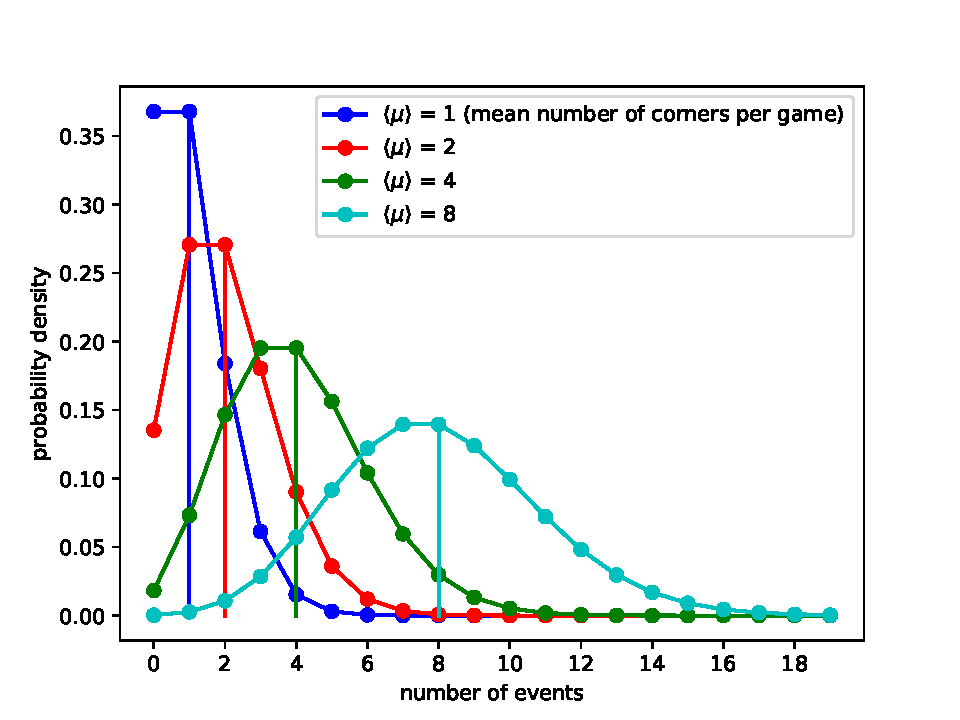
\includegraphics[scale=1.0,angle=0,trim=0cm 0cm 0cm 0cm]{fig_poison.pdf}
\caption{Example Poisson distributions for a selection of expected $\mu$ values. Vertical lines and the legend indicate the value of $\mu$.}
\label{fig_poison}
\end{center}
\end{figure} 





\subsection{Inter-team customisation}

It is insufficient to assume global means $\langle \mu_i \rangle$ and $\langle \mu_j \rangle$ for all the teams based on the global average of home corners and away corners in the training data. The model must account for the performance of specific teams against other specific teams. In other words, not all teams are equally skilled at attacking or defending and the expected number of corners will therefore depend on which two teams are playing. To improve the models flexibility and account for a teams previous performance from the training data, I introduce modifiers $\alpha$ and $\beta$ that modify the Poisson distribution's global mean according to each teams specific attack strength and defensive weakness.

The joint probability distribution $P_{ij}(n_i,n_j)$ of the home team $i$ scoring $n_i$ corners, and away team $j$ scoring $n_j$ corners is then

\begin{equation}
\label{eq_modpoison}
P_{ij}(n_i,n_j) = P_i(n_i|\mu_i) P_j(n_j|\mu_j),
\end{equation}

\noindent where the modified mean for the home $\mu_i$ and away $\mu_j$ teams are given by 

\begin{equation}
\mu_i = \langle \mu_i \rangle \alpha_i \beta_j,
\end{equation}

\noindent and

\begin{equation}
\mu_j = \langle \mu_j \rangle \alpha_j \beta_i,
\end{equation}

\noindent The modified mean for the home team $\mu_i$ is a function of the attacking strength of the home team $\alpha_i$ and the defensive weakness of the away team $\beta_j$ which respectively measure the fraction of corners won or conceded above the global $\mu_i$ such that

\begin{equation}
\label{eq_attack_home}
\alpha_i = \frac{\left( N(h_\mathrm{win}) / N(h_\mathrm{play} )\right) }{\langle \mu_i \rangle } 
\end{equation}

\noindent where $N(h_\mathrm{win})$ and $N(h_\mathrm{play})$ are the number of home corners won and number of home games played respectively. A corresponding equation for the attach strength of the away team exists such that

\begin{equation}
\label{eq_attack_away}
\alpha_j = \frac{\left( N(a_\mathrm{win}) / N(a_\mathrm{play}) \right) }{\langle \mu_j \rangle }.
\end{equation}


Finally, the defensive weaknesses are given by similar expressions such that

\begin{equation}
\label{eq_defend_home}
\beta_i = \frac{\left( N(h_\mathrm{concede}) / N(h_\mathrm{play}) \right) }{\langle \mu_i \rangle },
\end{equation}

\noindent and

\begin{equation}
\label{eq_defend_home}
\beta_j = \frac{\left( N(a_\mathrm{concede}) / N(a_\mathrm{play}) \right) }{\langle \mu_j \rangle },
\end{equation}

\noindent represent the number of corners conceded as a fraction of the global average for the home and away sides respectively.

\subsection{Use of League ID}
If, for a particular reason, a team has played no home games, use the mean value $\langle \alpha_i \rangle$ and $\langle \beta_i \rangle$ computed from home games within the same league. Similarly, for teams that have not played any away games, I use the mean value $\langle \alpha_j \rangle$ and $\langle \beta_j \rangle$ computed from away games within the same league. Figure xx in the appendix (feel free to skip over this) shows how the attach and defence strengths vary from league to league. It can be seen in this case that these are consistent with the global average ($\alpha$ and $\beta$ are scattered around one) so the required inter league calibration should be minimal in this case.


\subsection{Computation}
The quantities $\alpha_i$, $\alpha_j$, $\beta_i$, $\beta_j$, along with the global means for the home $\langle \mu_i \rangle$ and away $\langle \mu_j \rangle$ corners are computed from the training data set using the python script. Each game in the test set is then considered in turn within a `for' loop.  For each entry in the loop (each game), Equation \ref{eq_modpoison} is used to compute the probability of $n_i$ home corners and $n_j$ away corners $P_{ij}(n_i,n_j)$ up to a total of 20 home and 20 away corners (since the Poisson distribution is infinite, a cut-off must be imposed to ensure the code runs in a finite time). The probability that the total number of corners is below $P_b$, at $P_at$ or above $P_a$ the bet line $l$ is then calculated as 

\begin{equation}
\label{eq_pbelow}
P_b = \frac{\sum_{i+j < l} P_{ij}} {sum_{ij} P_{ij}},
\end{equation}

\begin{equation}
\label{eq_pat}
P_{at} = \frac{\sum_{i+j = l} P_{ij}} {sum_{ij} P_{ij}},
\end{equation}

\noindent and 

\begin{equation}
\label{eq_pabove}
P_a = \frac{\sum_{i+j < l} P_{ij}} {sum_{ij} P_{ij}}.
\end{equation}





\subsection{Bets}
In general, the expectation value of a random variable $X$ is given by 

\begin{equation}
E(X) = \int_{-\infty}^{\infty} X P(X) dX.
\end{equation}

In this case, we have the option of betting that the number of corners is above some specified fiducial value (a line) or below the line. The expected profit $E_a$ from a bet above the line is given by 

\begin{equation}
\label{eq_exp_above}
E_a = S \left(  \left[ O_a - 1 \right] P_a + \left[ -1 \right] P_b + \left[ O_{at} P_{at} \right]  \right),
\end{equation}

\noindent where $O_a$, $O_b$ and $O_\mathrm{at}$ are the bet odds given that the number of corners is above, below or at the line respectively. Since a push bet (where the results is at the line) returns the stake to the better, the final term disappears. This collapses to 
  
\begin{equation}
\label{eq_exp_above_simp}
E_a = S \left(  \left[ O_a - 1 \right] P_a - P_b  \right).
\end{equation}

\noindent where $S$ is the stake. Similarly, the expectated return on a bet under the line is given by 

\begin{equation}
\label{eq_exp_below}
E_b = S \left(  \left[ O_b - 1 \right] P_b + \left[ -1 \right] P_a + \left[ O_{at} P_{at} \right]  \right),
\end{equation}

\noindent which simplifies to

\begin{equation}
\label{eq_exp_below_simp}
E_b = S \left(  \left[ O_b - 1 \right] P_b - P_a  \right).
\end{equation}







\noindent The expected return from bets above $E_a$ and below $E_b$ the line are computed using Equations \ref{eq_exp_above_simp} and \ref{eq_exp_below_simp}. I bet either above the line, below the line or choose not to bet. The condition for a bet above the line is

\begin{equation}
\label{eq_abovebet_condition}
E_a > E_b > 0,
\end{equation}

\noindent and, for below the line,
\begin{equation}
\label{eq_belowbet_condition}
E_b > E_a > 0.
\end{equation}


\noindent If none of these conditions are obeyed, no bet is placed. I then move on to the next game in the loop.
 
 
 
 






\section{Results}
\label{sec_res}


The algorithm described in Sections \ref{sec_method} is executed in a Python script to compute the quantities $\alpha_i$, $\alpha_j$, $\beta_i$, $\beta_j$, along with the global means for the home $\langle \mu_i \rangle$ and away $\langle \mu_j \rangle$. The trained model then iterates through each game in the test data set to compute $P_a$, $P_{at}$, $P_b$, $E_a$ and $E_b$. The results are then used to assign the bet according to Equations \ref{eq_abovebet_condition} and \ref{eq_belowbet_condition}. The accompanying csv \verb|test_op.csv| file lists each of these quantities for each game in the test set as requested. 





\begin{figure}
\begin{center}
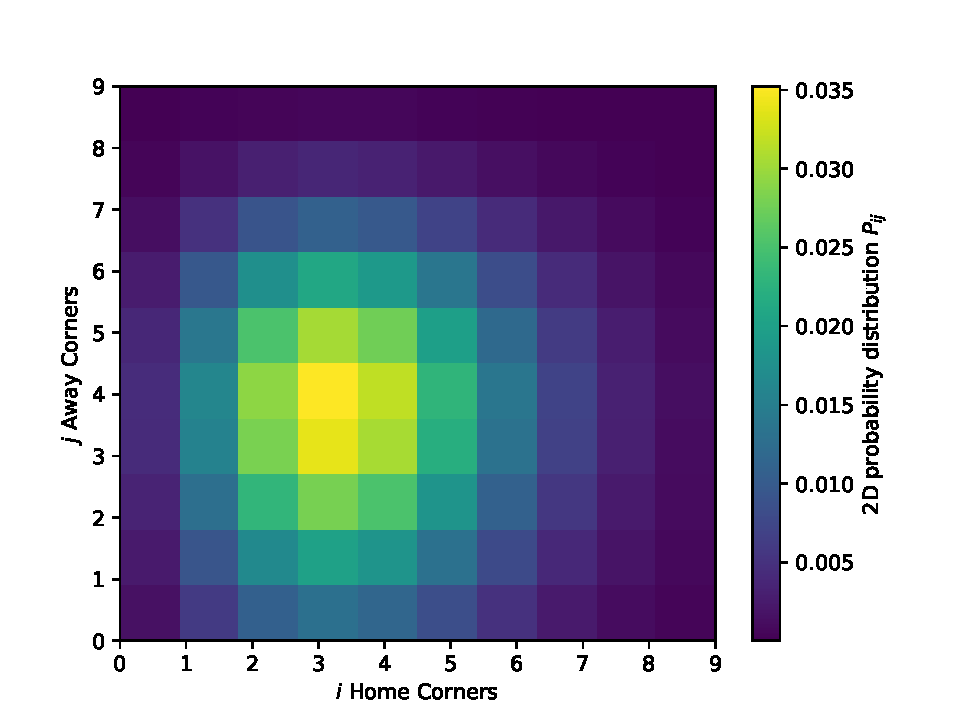
\includegraphics[scale=1.0,angle=0,trim=0cm 0cm 0cm 0cm]{fig_eg_posterior.pdf}
\caption{Example posterior probability distributions for an example from game ID 341 from the test sample. The 2D posterior probability distributions are computed using Equation \ref{eq_modpoison}. }
\label{fig_posterior_eg}
\end{center}
\end{figure} 


\section{Future Potential Improvements}
Given additional time, one could note that the attack and defence modifiers for the home and away teams $\alpha_i$, $\alpha_j$ and $\beta_i$ and $\beta_j$ may change with time. Teams may get better or worse under new management or as players are transferred away or join a team. In modelling this 5-year data set, it is assumed these quantities are constant. One could test this by computing the global means of home and away corners $\langle \mu_i \rangle$ and $\langle \mu_j \rangle$ for each season and noting if these exhibit significant variations outside their root-mean-square (RMS) scatter (Figure \ref{fig_league_ave}).

It is also possible to test the models' accuracy by dividing the training data into a subset of training and test data. The new `test' data, derived from the original training sample, will have actual results to compare against the model predictions. The expected betting profit from such a model can be calculated so long as lines and profits are provided just as with the test sample. Splitting the training data in this way is known as `cross validation' and simply requires the lines and odds for the training sample to be provided. Cross validation then provides a diagnostic and predicted performance of the model before applying to real data.

One could also apply neural nets to study the past match history of individual combinations of teams (e.g Liverpool Vs Man-u) to study how more subtle attributes affect the game performance (day of the week, weather conditions etc). The `importance' of the match may also be a factor that could be studied on an individual case basis. For example perhaps Man-u cope better under pressure than Liverpool, who may be more likely to `bottle it' in a high profile game like a final match but may do better in a low-stakes friendly match.  

All these scenarios could form the basis of future studies and improve the accuracy and generality of the fitted model.

Thank you for taking the time to consider my project and application.






\section{Appendix}

\begin{figure}[h]
\begin{center}
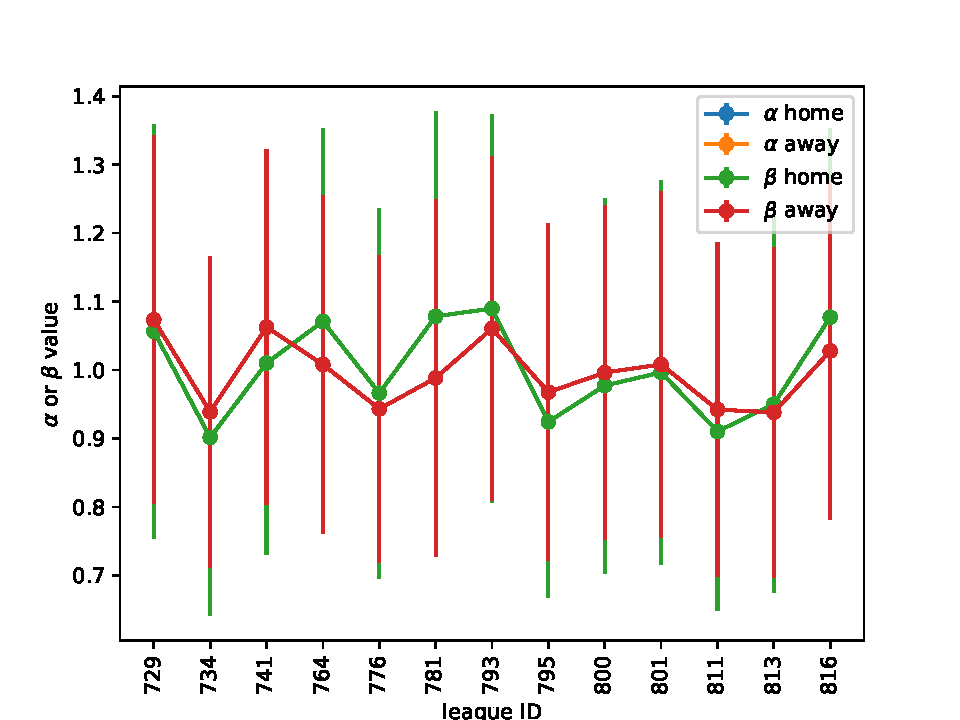
\includegraphics[scale=1.0,angle=0,trim=0cm 0cm 0cm 0cm]{fig_alpha_beta_league_ave.pdf}
\caption{Variation in attack $\alpha$ and defence $\beta$ strength averages for teams in different leagues. A value of 1 means the attack or defence strength is consistent with the global average.}
\label{fig_league_ave}
\end{center}
\end{figure} 

\end{document}



